\chapter{Metodología}
\section{Introducción}

La finalidad de definir desde el principio una metodoligía y hacer uso de esta durante todo el desarrollo es la de hacer más eficaz el proceso de desarrollo del producto y lograr una alta calidad de forma que sea costeable tanto para el equipo de trabajo como para el cliente mismo, la metodología también define las reglas de trabajo para el grupo que llevara a cabo el desarrollo, las actividades y los procesos que este grupo debe realizar y la forma en que debe realizarlos.
\newline
Para este caso en especifico se busca una metodología de trabajo que principalmente incluya al cliente como una de las partes fundamentales del desarrollo y permita al equipo estar en constante comunicación con este, la metodología debe permitir atender requerimientos emergentes y ademas la metodología escogida debe permitir mostrar al cliente los avances desarrollados en un período de tiempo de forma que este pueda hacer comentarios y exprese su satisfacción o informe en caso de que no este conforme con algo.
\newpage

\section{Prototipo}
Para el desarrollo de la plataforma web, se utilizara la metodología "Prototipo para desarrollo del software", la cual consta de una fase de requerimientos y de diseño con la creación de un subproducto, es esto lo que llamamos prototipo ya que es una fase temprana del mismo para ver su comportamiento, posteriormente se realiza una fase de implementación, una pruebas y una final de mantenimiento.
\newline
Además de esto se escoge esta metodología puesto que esta permite al cliente ser parte del proceso de desarrollo viendo el avance que este lleva y haciendo las observaciones pertinentes desde su punto de vista, de forma que se crea un dialogo entre el equipo de desarrollo y el cliente que permite establecer mejor las funcionalidades que se espera tenga el producto final y los requisitos que debe cumplir. Esto mejora la calidad del producto asegurando que este cumpla con las expectativas del cliente.
\begin{figure}[th!]
	\centering
	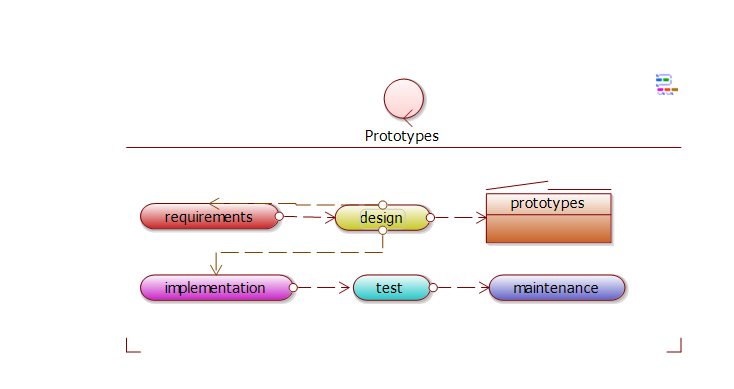
\includegraphics[width=0.9\linewidth]{imagenes/Proceso1}
	\caption{Proceso de desarrollo de software: Prototipo}
\end{figure}

\newpage

\section{Cronograma}

Teniendo claro la metodología a utilizar, se procede a organizar el tiempo requerido para realizar el desarrollo del proyecto, teniendo en cuenta la cantidad de semanas destinadas para el desarrollo completo del prototipo y la documentación pertinente.


\newpage